\documentclass[aps,prb,twocolumn,superscriptaddress,floatfix,longbibliography]{revtex4-2}

\usepackage[utf8]{inputenc}
\usepackage[spanish]{babel}
\usepackage{graphicx}
\usepackage{amsmath}
\usepackage{subcaption}
\usepackage{wrapfig} 
\usepackage[export]{adjustbox}

\usepackage{amsmath,amssymb} % math symbols
\usepackage{bm} % bold math font
\usepackage{graphicx} % for figures
\usepackage{comment} % allows block comments
\usepackage{textcomp} % This package is just to give the text quote '
\usepackage{listings} %para agregar codigo

%\usepackage{ulem} % allows strikeout text, e.g. \sout{text}

\usepackage[spanish]{babel}

\usepackage{enumitem}
\setlist{noitemsep,leftmargin=*,topsep=0pt,parsep=0pt}

\usepackage{xcolor} % \textcolor{red}{text} will be red for notes
\definecolor{lightgray}{gray}{0.6}
\definecolor{medgray}{gray}{0.4}

\usepackage{hyperref}
\hypersetup{
colorlinks=true,
urlcolor= blue,
citecolor=blue,
linkcolor= blue,
bookmarks=true,
bookmarksopen=false,
}

% Code to add paragraph numbers and titles
\newif\ifptitle
\newif\ifpnumber
\newcounter{para}
\newcommand\ptitle[1]{\par\refstepcounter{para}
{\ifpnumber{\noindent\textcolor{lightgray}{\textbf{\thepara}}\indent}\fi}
{\ifptitle{\textbf{[{#1}]}}\fi}}
%\ptitletrue  % comment this line to hide paragraph titles
%\pnumbertrue  % comment this line to hide paragraph numbers

% minimum font size for figures
\newcommand{\minfont}{6}

% Uncomment this line if you prefer your vectors to appear as bold letters.
% By default they will appear with arrows over them.
% \renewcommand{\vec}[1]{\bm{#1}}

%Cambiar Cuadros por Tablas y lista de...
%\renewcommand{\listtablename}{indice de tablas}
\renewcommand{\tablename}{Tabla}
\renewcommand{\date}{Fecha}

% \graphicspath{ {C:/Users/lupam/Mi unidad/Pablo Chehade/Instituto Balseiro (IB)/Laboratorio Avanzado/Informe/V5/Figures} } %Para importar imagenes desde una carpeta


\lstset{
  basicstyle=\ttfamily\small,
  breaklines=true,
  frame=single,
  numbers=left,
  numberstyle=\tiny,
  keywordstyle=\color{blue},
  commentstyle=\color{green},
  stringstyle=\color{red},
} %Configuración para el bloque de código


\usepackage[bottom]{footmisc} %para que las notas al pie aparezcan en la misma pagina



\begin{comment}

%Comandos de interes:

* Para ordenar el documento:
\section{Introducción}
\section{\label{sec:Formatting}Formatting} %label para luego hacer referencia a esa sección

\ptitle{Start writing while you experiment} %pone nombre y título al documento dependiendo de si en el header están los comandos \ptitletrue y \pnumbertrue

* Ecuaciones:
\begin{equation}
a^2+b^2=c^2 \,.
\label{eqn:Pythagoras}
\end{equation}

* Conjunto de ecuaciones:
\begin{eqnarray}
\label{eqn:diagonal}
\nonumber d & = & \sqrt{a^2 + b^2 + c^2} \\
& = & \sqrt{3^2+4^2+12^2} = 13
\end{eqnarray}

* Para hacer items / enumerar:
\begin{enumerate}
  \item
\end{enumerate}

\begin{itemize}
  \item
\end{itemize}

* Figuras:
\begin{figure}[h]
    \includegraphics[clip=true,width=\columnwidth]{pixel-compare}
    \caption{}
     \label{fig:pixels}
\end{figure}

* Conjunto de figuras:
(no recuerdo)


* Para hacer referencias a fórmulas, tablas, secciones, ... dentro del documento:
\ref{tab:spacing}

* Para citar
Elementos de .bib
\cite{WhitesidesAdvMat2004}
url
\url{http://www.mendeley.com/}\\

* Agradecimientos:
\begin{acknowledgments}
We acknowledge advice from Jessie Zhang and Harry Pirie to produce Fig.\ \ref{fig:pixels}.
\end{acknowledgments}

* Apéndice:
\appendix
\section{\label{app:Mendeley}Mendeley}

* Bibliografía:
\bibliography{Hoffman-example-paper}

\end{comment}


\begin{document}

% Allows to rewrite the same title in the supplement
\newcommand{\mytitle}{Memorias Asociativas}

\title{\mytitle}

\author{Pablo Chehade \\
    \small \textit{pablo.chehade@ib.edu.ar} \\
    \small \textit{Redes Neuronales, Instituto Balseiro, CNEA-UNCuyo, Bariloche, Argentina, 2023} \\}
    
\maketitle


\section*{Ejercicio 1}



Se calculó la dinámica de una red de Hopfield sin ruido con regla de actualización secuencial y paralela para tamaños de red \( N = 500, 1000, 2000, 4000 \) y para valores de \( \alpha = \frac{p}{N} = 0.12, 0.14, 0.16, 0.18 \), con $p$ número de patrones. En cada red, se realizaron \( p \) simulaciones donde se tomó como condición inicial cada uno de los patrones aleatorios $\xi^\mu$ y se iteró la dinámica hasta converger a un punto fijo \( s_i^{\mu} \). La convergencia fue evaluada mediante la comparación de la configuración de la red en un tiempo grande \( t \) con su estado en \( t+1 \).

En base a los resultados, se calculó la fracción de simulaciones convergidas (\( f_{conv} \)) para la iteración secuencial y paralela variando $N$ y $\alpha$. Los resultados se resumen en las tablas \ref{tab:ej1_f_conv_secuencial} y \ref{tab:ej1_f_conv_paralela}.

% Tabla de f_conv para iteración secuencial
\begin{table}[h]
  \centering
  \caption{Fracción de simulaciones convergidas (\( f_{conv} \)) para iteración secuencial}
  \label{tab:ej1_f_conv_secuencial}
  \begin{tabular}{|c|c|c|c|c|}
  \hline
  \( N \) \ \( \alpha \) & 0.12   & 0.14   & 0.16   & 0.18   \\ \hline
  500            & 1.0000 & 1.0000 & 1.0000 & 1.0000 \\ \hline
  1000           & 1.0000 & 1.0000 & 1.0000 & 1.0000 \\ \hline
  2000           & 1.0000 & 1.0000 & 1.0000 & 1.0000 \\ \hline
  4000           & 1.0000 & 1.0000 & 1.0000 & 1.0000 \\ \hline
  \end{tabular}
\end{table}
  
% Tabla de f_conv para iteración paralela
\begin{table}[h]
  \centering
  \caption{Fracción de simulaciones convergidas (\( f_{conv} \)) para iteración paralela}
  \label{tab:ej1_f_conv_paralela}
  \begin{tabular}{|c|c|c|c|c|}
  \hline
  \( N \) \ \( \alpha \) & 0.12   & 0.14   & 0.16   & 0.18   \\ \hline
  500            & 0.9667 & 0.9143 & 0.7125 & 0.5000 \\ \hline
  1000           & 0.9333 & 0.8643 & 0.4062 & 0.1111 \\ \hline
  2000           & 0.9625 & 0.7071 & 0.2437 & 0.0306 \\ \hline
  4000           & 0.8875 & 0.5250 & 0.0688 & 0.0000 \\ \hline
  \end{tabular}
\end{table}
  

Se observó una completa convergencia $f_{conv} = 1$ en la dinámica secuencial para todos los valores de \( N \) y \( \alpha \). En contraste, la dinámica paralela mostró una disminución progresiva en la convergencia con el aumento de \( \alpha \) y el tamaño de la red \( N \).

Además, para la dinámica secuencial, se calculó el overlap \( m^{\mu} \) definido como

\[ m^{\mu} = \frac{1}{N} \sum_{i=1}^{N} s_i^{\mu} \xi_i^{\mu} \]

Este overlap mide la similitud entre el punto fijo \( s^{\mu} \) y el patrón original \( \xi^{\mu} \). Teóricamente, se espera que para \( \alpha = 0 \), el overlap inicie en 1 y decrezca lentamente con el incremento de \( \alpha \), alcanzando un valor de aproximadamente $0.97$ para \( \alpha = 0.14 \). A partir de este punto, se espera una caída abrupta del overlap.

Los histogramas de overlap para diferentes condiciones iniciales confirmaron parcialmente las expectativas teóricas, como se observa en la figura \ref{fig:ej1_histograma}.
\begin{itemize}
  \item Para \( \alpha < 0.14 \), el overlap es cercano a 1, indicando que la red es capaz de recordar de manera correcta los patrones.
  \item Para \( \alpha = 0.14 \), el overlap es menor pero cercano a 1.
  \item Para \( \alpha > 0.14 \), el overlap disminuye significativamente.
\end{itemize}

Sin embargo, no se observó una caída abrupta a cero después de \( \alpha = 0.14 \), sino a valores alrededor de $0.3$, lo cual puede atribuirse a la presencia de estados metaestables en la red.


\begin{figure}[h]
  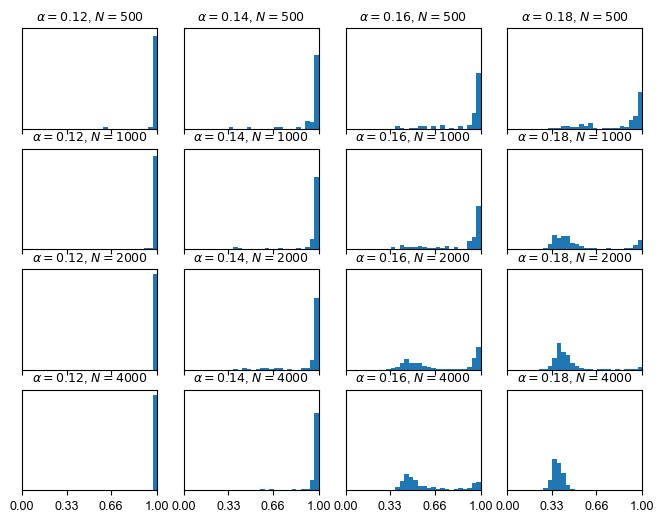
\includegraphics[clip=true,width=\columnwidth]{../ej1_histograma.png}
  \caption{}
   \label{fig:ej1_histograma}
\end{figure}

\section*{Ejercicio 2}

Se simuló la dinámica de una red de Hopfield en presencia de ruido, utilizando la regla de actualización estocástica
\[ Pr(s_i(t + 1) = \pm1) = \frac{\exp(\pm\beta h_i(t))}{\exp(\beta h_i(t)) + \exp(-\beta h_i(t))}, \]
donde \( h_i(t) = \sum_{j=1}^{N} w_{ij}s_j(t) \). Para esta simulación, se empleó dimensión \( N = 4000 \) y \( p = 40 \) patrones, resultando en un valor de \( \alpha = p/N = 0.01 \), cercano a cero. Se exploraron temperaturas \( T = \frac{1}{\beta} \) variando desde $0.1$ hasta $2$ en incrementos de $0.1$.

Se realizaron $p$ simulaciones empleando como condición inicial cada uno de los patrones \( \xi_i^\mu \). La regla de actualización se aplicó iterativamente diez veces en cada sitio de la red. A partir de estas iteraciones, se calculó el overlap medio, definido como:
\[ m^\mu = \frac{1}{N} \sum_{j=1}^{N} \langle S_j(t) \rangle \xi_j^\mu, \]
donde el promedio \( \langle \ldots \rangle \) se calculó sobre la dinámica.

En la figura \ref{fig:ej2_overlap_vs_T} se grafica el overlap medio en función de la temperatura. Los resultados muestran el comportamiento esperado con un overlap medio \( m^\mu \) igual a 1 para \( T = 0 \), de acuerdo con los resultados del ejercicio previo. A medida que la temperatura aumenta, el overlap medio disminuye progresivamente, lo cual está de acuerdo con la teoría. No obstante, en lugar de anularse completamente a \( T = 1 \), el overlap medio mantuvo un valor residual y continuó disminuyendo para temperaturas superiores. Esto puede deberse al tamaño finito del sistema.

\begin{figure}[h]
  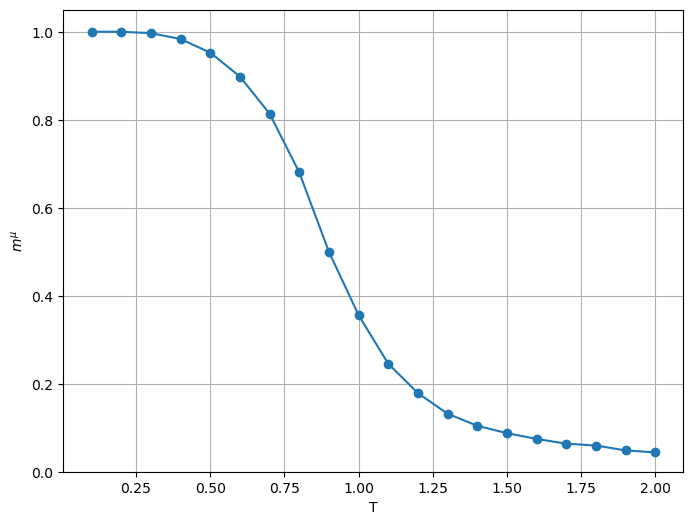
\includegraphics[clip=true,width=\columnwidth]{../ej2_overlap_vs_T.png}
  \caption{}
   \label{fig:ej2_overlap_vs_T}
\end{figure}





\onecolumngrid


\section*{Apéndice}
A continuación se desarrolla el código empleado durante este trabajo implementado en Python.




\begin{lstlisting}[language=Python]
    

  #Import libraries
  import numpy as np
  import matplotlib
  import matplotlib.pyplot as plt
  from tqdm.notebook import tqdm
  
  # ## Ejercicio 1
  alpha_vec = np.array([0.12, 0.14, 0.16, 0.18])
  N_vec = np.array([500, 1000, 2000, 4000])
  # alpha_vec = np.array([0.18])
  # N_vec = np.array([500])
  # N_vec = np.array([50, 100, 200, 400])
  alpha = alpha_vec[0] #valor tipico a usar en las simulaciones
  N = N_vec[0] #valor tipico a usar en las simulaciones
  
  #Calculo p
  p = int(alpha*N)
  print(f"p = {p}")
  
  def gen_patrones(p, N):
      #Se generan p patrones de N elementos. Se retornan como una matriz
      return np.random.randint(0,2, size = (p, N))*2 - 1
  #Calculo la matriz de conexiones
  
  def matriz_conexiones(x):
      #x: patrones
      #Menos eficiente:
      W = np.zeros((N,N))
      #Calculo el producto externo
      for mu in range(p):
          W += np.outer(x[mu], x[mu])
      #Se eliminan las conexiones de la neurona consigo misma
      W -= np.diag(np.diag(W))
  
      #De forma mas eficiente:
      # W = np.einsum('...i,...j->...ij', x, x).sum(axis=0)
      # np.fill_diagonal(W, 0)
  
      return W/x.shape[1]
  
  # matriz_conexiones(gen_patrones(5, 5))
  def iter_secuencial_determinista(S_t, W, T = 0):
      #Calcula S(t+1) dado S(t) de forma secuencial
      for i in range(N):
          S_t[i] = np.sign(np.dot(W[i], S_t))
  
      return S_t
  
  def iter_paralelo_determinista(S_t, W, T = 0):
      #Calcula S(t+1) dado S(t) de forma paralela
      S_t_new = np.sign(np.dot(W, S_t))
  
      return S_t_new
  
  #Def la funcion de Lyapunov
  def E_Lyapunov(S, W):
      #S: configuracion de la red
  
      return -1/2*np.sum(W*np.outer(S, S))
  
  def overlap_determinista(S_matrix, x):
      #Calcula el overlap entre s y x
      return np.dot(S_matrix[-1], x)/N
  
  def evolution(p, N, iter_, overlap, T = 0, N_iter = 10, calculate_all = False):
      #iter_: funcion que calcula la dinamica de la red. Como input tiene S(t) y W
      #overlap: funcion que calcula el overlap entre S(t_final) y x
      #calculate_all indica si se calcula el error y delta_S
  
      x = gen_patrones(p, N)
      W = matriz_conexiones(x)
  
      # print(f"Matrix W: {W}")
  
      overlap_vec = np.empty(p)
      f_conv_vec = np.empty(p)
  
      if calculate_all:
          error_matrix = np.empty([p, N_iter])
          delta_S_matrix = np.empty([p, N_iter - 1])
          
  
      for mu in range(p):
  
          S_matrix = np.empty([N_iter, N])
          #CI
          S_matrix[0] = x[mu] #np.random.randint(0,2, size = (N))*2 - 1
  
          for t in range(1, N_iter):
              S_matrix[t] = iter_(S_matrix[t-1], W, T)
              # print(f"Iter: {t}, suma = {np.sum(S_matrix[t-1]*S_matrix[t])}")
          
  
          f_conv_vec[mu] = np.all(S_matrix[-2] == S_matrix[-1]) #fraccion de simulaciones que convergieron
          
          overlap_vec[mu] = overlap(S_matrix, x[mu])
          #Control
          # if overlap_vec[mu] < 0 or overlap_vec[mu] > 1:
              # raise ValueError(f"El overlap es {overlap_vec[mu]}")
  
          if calculate_all:
              delta_S_array = np.mean(np.abs(S_matrix[1:] - S_matrix[:-1]), axis = 1)
              delta_S_matrix[mu] = delta_S_array
              error_array = np.mean(np.abs(S_matrix - S_matrix[0])**2, axis = 1)
              error_matrix[mu] = error_array
  
      if calculate_all:
          #Calculo el valor medio del error
          delta_S_medio = np.mean(delta_S_matrix, axis = 0)
          delta_S_std = np.std(delta_S_matrix, axis = 0)/np.sqrt(p) #desviacion estandard de la media
          error_medio = np.mean(error_matrix, axis = 0)
          error_std = np.std(error_matrix, axis = 0)/np.sqrt(p) #desviacion estandard de la media
  
      #Calculo cuantas veces convergio
      #es decir, cuantas veces delta_S_matrix[:, -2] - delta_S_matrix[:,-1] == 0
  
  
      if calculate_all:
          return delta_S_medio, delta_S_std, error_medio, error_std, overlap_vec, f_conv_vec
      else:
          return overlap_vec, np.mean(f_conv_vec)
  
  # N_iter = 20
  # delta_S_medio_seq, delta_S_std_seq, error_medio_seq, error_std_seq, overlap_vec_seq, f_conv_seq = evolution(p, N, iter_secuencial_determinista, overlap_determinista, N_iter = N_iter, calculate_all=True)
  # delta_S_medio_par, delta_S_std_par, error_medio_par, error_std_par, overlap_vec_par, f_conv_par = evolution(p, N, iter_secuencial_determinista, overlap_determinista, N_iter = N_iter, calculate_all=True)
  
  #Recorro N_vec y alpha_vec, calculo para cada caso f_conv y luego imprimo todos los valores en una tabla
  
  N_iter = 20
  
  f_conv_seq_matrix = np.empty([len(N_vec), len(alpha_vec)])
  f_conv_par_matrix = np.empty([len(N_vec), len(alpha_vec)])
  
  for i in tqdm(range(len(N_vec))):
      for j in range(len(alpha_vec)):
          N = N_vec[i]
          alpha = alpha_vec[j]
          p = int(alpha*N)
          # print(f"p = {p}")
  
          # overlap_vec_seq, f_conv_seq_matrix[i,j] = evolution(p, N, iter_secuencial_determinista, overlap_determinista, N_iter = N_iter, calculate_all=False)
          overlap_vec_par, f_conv_par_matrix[i,j] = evolution(p, N, iter_paralelo_determinista, overlap_determinista, N_iter = N_iter, calculate_all=False)
          
          #Guardo datos
          # np.save(f'resultados/ej1_overlap_vec_seq_{i}{j}', overlap_vec_seq)
  
  
  # np.save('resultados/ej1_f_conv_seq_matrix', f_conv_seq_matrix)
  np.save('resultados/ej1_f_conv_par_matrix', f_conv_par_matrix)
     
  
  # ## Ejercicio 2
  import random
  
  def iter_secuencial_estocastico(S_t, W, T):
      #Calcula S(t+1) dado S(t) de forma secuencial
  
      #Calculo beta
      beta = 1/T
  
      for i in range(N):
          #Calculo h_i
          h_i = np.dot(W[i], S_t)
          #Tiro un numero aleatorio
          aleatorio = random.random()
          #Calculo la probabilidad de que S_t[i] = 1
          Pr = np.exp(beta*h_i)/(np.exp(beta*h_i) + np.exp(-beta*h_i))
          if aleatorio < Pr:
              S_t[i] = 1
          else:
              S_t[i] = -1
  
      return S_t
  
  def overlap_estocastico(S_matrix, x):
      #Calculo el overlap entre <S> y x
  
      #Calculo <S>
      S_medio = np.mean(S_matrix, axis = 0)
  
      return np.dot(S_medio, x)/N
  
  N = 4000
  p = 40
  T_vec = np.linspace(0.1,2,20)
  
  overlap_mean_vec = np.empty(len(T_vec))
  overlap_std_vec = np.empty(len(T_vec))
  
  for i in tqdm(range(len(T_vec))):
      T = T_vec[i]
      overlap_vec, f_conv = evolution(p, N, iter_secuencial_estocastico, overlap_estocastico, T = T, N_iter = 10, calculate_all = False)
      overlap_mean_vec[i] = np.mean(overlap_vec)
      overlap_std_vec[i] = np.std(overlap_vec)/np.sqrt(p)
  
  
  #Guardo datos
  np.save('resultados/ej2_T_vec', T_vec)
  np.save('resultados/ej2_overlap_mean_vec', overlap_mean_vec)
  np.save('resultados/ej2_overlap_std_vec', overlap_std_vec)
  
  
  
  import numpy as np
  import matplotlib
  import matplotlib.pyplot as plt
  from tqdm.notebook import tqdm
  
  # ## Ejercicio 1
  alpha_vec = np.array([0.12, 0.14, 0.16, 0.18])
  N_vec = np.array([500, 1000, 2000, 4000])
  #Imprimo una tabla con los valores de f_col
  
  f_conv_seq_matrix = np.load("resultados/ej1_f_conv_seq_matrix.npy")
  f_conv_par_matrix = np.load("resultados/ej1_f_conv_par_matrix.npy")
  
  print("Tabla de f_conv para iteracion secuencial")
  print(r"N\alpha", end = '\t')
  for alpha in alpha_vec:
      print(f"{alpha:.2f}", end = '\t')
  print()
  for i in range(len(N_vec)):
      print(N_vec[i], end = '\t')
      for j in range(len(alpha_vec)):
          print(f"{f_conv_seq_matrix[i,j]:.4f}", end = '\t')
      print()
  
  
  print("Tabla de f_conv para iteracion paralela")
  print(r"N\alpha", end = '\t')
  for alpha in alpha_vec:
      print(f"{alpha:.2f}", end = '\t')
  print()
  for i in range(len(N_vec)):
      print(N_vec[i], end = '\t')
      for j in range(len(alpha_vec)):
          print(f"{f_conv_par_matrix[i,j]:.4f}", end = '\t')
      print()
  
  # Grafico un histograma de todos los overlaps
  
  fig, ax = plt.subplots(len(alpha_vec),len(N_vec), figsize = (8,6), sharex=True, sharey=True)
  
  for i in range(len(N_vec)):
      for j in range(len(alpha_vec)):
          alpha = alpha_vec[i]
          N = N_vec[j]
          p = int(alpha*N)
          overlap_vec = np.load(f"resultados/ej1_overlap_vec_seq_{i}{j}.npy")
  
          ax[i,j].hist(overlap_vec, range = (0,1), bins = 30, density = True)
          ax[i,j].set_xlim([0,1])
          #Agrego titulo de tamano 9
          ax[i,j].set_title( fr'$\alpha = {alpha_vec[j]}$, $N = {N_vec[i]}$', fontsize = 9)
          # ax[i,j].set_ylabel('Frecuencia')
          #Saco los ticks y labels del eje y
          ax[i,j].set_yticks([])
          ax[i,j].set_yticklabels([])
          #Uso tick labels en x en 0, 0.33, 0.66 y 1 con 2 decimales
          ax[i,j].set_xticks([0, 0.33, 0.66, 1])
          #Achico el tamano de los labels
          ax[i,j].tick_params(axis='x', labelsize=9)
          
  plt.show()
  
  #Guardo figura
  fig.savefig("ej1_histograma.png", bbox_inches='tight')
  
  #Guardo figura
  fig.savefig("ej1_overlap_mean.png", bbox_inches='tight')
  # ## Ejercicio 2
  #Cargo datos
  T_vec = np.load("resultados/ej2_T_vec.npy")
  overlap_mean_vec = np.load("resultados/ej2_overlap_mean_vec.npy")
  # overlap_std_vec = np.load("resultados/ej2_overlap_std_vec.npy")
  #Grafico overlap en funcion de T
  
  fig, ax = plt.subplots(1,1, figsize = (8,6))
  
  # ax.errorbar(T_vec, overlap_mean_vec, yerr = overlap_std_vec, fmt = 'o-', capsize = 5)
  ax.plot(T_vec, overlap_mean_vec, '-o', color = 'tab:blue')
  ax.set_xlabel('T')
  ax.set_ylabel(r'$m^\mu$')
  ax.set_ylim([0,1.05])
  ax.grid()
  
  plt.show()
  
  #Guardo la figura
  fig.savefig("ej2_overlap_vs_T.png", bbox_inches='tight')
  
  
  
  
\end{lstlisting}

\bibliography{Chehade_practica_6.bib}

\end{document}





